\chapter{拉丁转写对照}
本附录参考维基百科罗列了希腊语,俄语和日语的拉丁转写,并以各国数学家人名为例,具体参照

\url{https://mathpron.github.io}

本附录采用宽式IPA,有关国际音标(IPA)的内容请参考\cite{LT}以及

\url{https://en.wikipedia.org/wiki/International_Phonetic_Alphabet}

\url{https://www.bilibili.com/video/BV1QA411i7Yf}

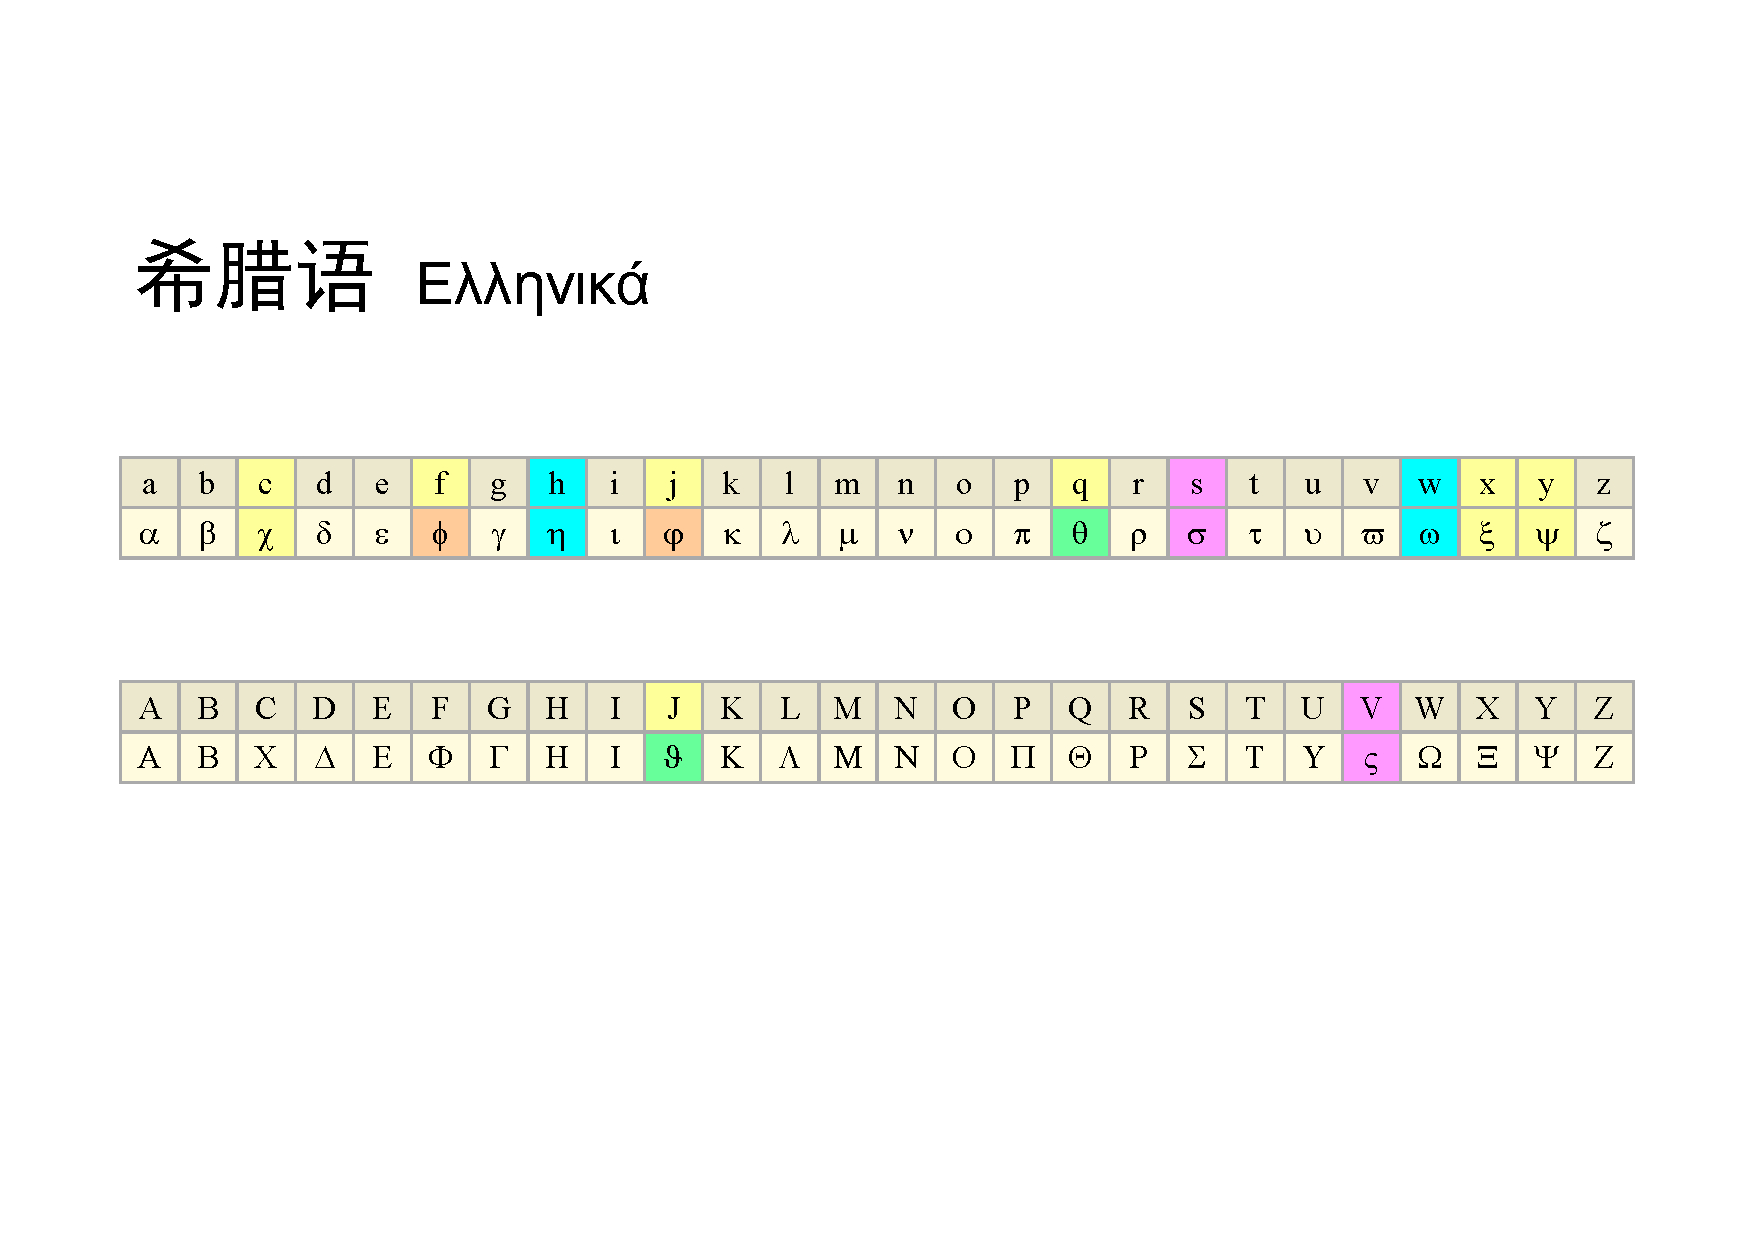
\includepdf[pagecommand={\thispagestyle{plain}},pages=-]{lin}
%addtotoc={{1,2},{希腊语},1,{希腊语},{Greek}}